%\renewcommand{\theequation}{\theenumi}
%\begin{enumerate}[label=\arabic*.,ref=\thesubsection.\theenumi]
%\numberwithin{equation}{enumi}
\item Find the coordinates of the point which divides the join of 
\begin{align}
\myvec{-1\\7},  \myvec{4\\-3}
%\vec{P} = \myvec{2\\-3}, \vec{Q} = \myvec{10\\y}
\end{align}
%
in the ratio $2:3$.
\\
\solution
Let the balanced version of (\ref{eq:solutions/chem/6ato balance}) be
\begin{align}
    \label{eq:solutions/chem/6abalanced}x_{1}HNO_{3}+ x_{2}Ca(OH)_{2}\to x_{3}Ca(NO_{3})_{2}+ x_{4}H_{2}O
\end{align}

which results in the following equations:
\begin{align}
    (x_{1}+ 2x_{2}-2x_{4}) H= 0\\
    (x_{1}-2x_{3}) N= 0\\
    (3x_{1}+ 2x_{2}-6x_{3}- x_{4}) O=0\\
    (x_{2}-x_{3}) Ca= 0
\end{align}

which can be expressed as
\begin{align}
    x_{1}+ 2x_{2}+ 0.x_{3} -2x_{4} = 0\\
    x_{1}+ 0.x_{2} -2x_{3} +0.x_{4}= 0\\
    3x_{1}+ 2x_{2}-6x_{3}- x_{4} =0\\
    0.x_{1} +x_{2}-x_{3} +0.x_{4}= 0
\end{align}

resulting in the matrix equation
\begin{align}
    \label{eq:solutions/chem/6a matrix}
    \myvec{1 & 2 & 0 & -2\\
           1 & 0 & -2 & 0\\
           3 & 2 & -6 & -1\\
           0 & 1 & -1 & 0}\vec{x}
           =\vec{0}
\end{align}

where,
\begin{align}
   \vec{x}= \myvec{x_{1}\\x_{2}\\x_{3}\\x_{4}}
\end{align}

(\ref{eq:solutions/chem/6a matrix}) can be reduced as follows:
\begin{align}
    \myvec{1 & 2 & 0 & -2\\
           1 & 0 & -2 & 0\\
           3 & 2 & -6 & -1\\
           0 & 1 & -1 & 0}
    \xleftrightarrow[R_{3}\leftarrow \frac{R_3}{3}-R_{1}]{R_{2}\leftarrow R_2- R_1}
    \myvec{1 & 2 & 0 & -2\\
           0 & -2 & -2 & 2\\
           0 & -\frac{4}{3} & -2 & \frac{5}{3}\\
           0 & 1 & -1 & 0}\\
    \xleftrightarrow{R_2 \leftarrow -\frac{R_2}{2}}
    \myvec{1 & 2 & 0 & -2\\
          0 & 1 & 1 & -1\\
          0 & -\frac{4}{3} & -2 & \frac{5}{3}\\
          0 & 1 & -1 & 0}\\
    \xleftrightarrow[R_4 \leftarrow R_4- R_2]{R_3 \leftarrow R_3 + \frac{4}{3}R_2}
    \myvec{1 & 2 & 0 & -2\\
           0 & 1 & 1 & -1\\
           0 & 0 & -\frac{2}{3} & \frac{1}{3}\\
           0 & 0 & -2 & 1}\\
    \xleftrightarrow[R_3 \leftarrow -\frac{3}{2}R_3]{R_1 \leftarrow R_1- 2R_2}
    \myvec{1 & 0 & -2 & 0\\
           0 & 1 & 1 & -1\\
           0 & 0 & 1 & -\frac{1}{2}\\
           0 & 0 & -2 & 1}\\
    \xleftrightarrow{R_4\leftarrow R_4 + 2R_3}
    \myvec{1 & 0 & -2 & 0\\
           0 & 1 & 1 & -1\\
           0 & 0 & 1 & -\frac{1}{2}\\
           0 & 0 & 0 & 0}\\
    \xleftrightarrow[R_2\leftarrow R_2-R_3]{R_1\leftarrow R_1 + 2R_3}
    \myvec{1 & 0 & 0 & -1\\
           0 & 1 & 0 & -\frac{1}{2}\\
           0 & 0 & 1 & -\frac{1}{2}\\
           0 & 0 & 0 & 0}
\end{align}

Thus,
\begin{align}
    x_1=x_4, x_2= \frac{1}{2}x_4, x_3=\frac{1}{2}x_4\\
    \implies \quad\vec{x}= x_4\myvec{1\\ \frac{1}{2}\\ \frac{1}{2}\\1} =\myvec{2\\1\\1\\2}
\end{align} 
by substituting $x_4= 2$.

\hfill\break
%\vspace{5mm} 
Hence, (\ref{eq:solutions/chem/6abalanced}) finally becomes
\begin{align}
    2HNO_{3}+ Ca(OH)_{2}\to Ca(NO_{3})_{2}+ 2H_{2}O
\end{align}


\item Find the coordinates of the points of trisection of the line segment joining \myvec{4\\-1} and \myvec{-2\\-3}.
\\
\solution
Let the balanced version of (\ref{eq:solutions/chem/6ato balance}) be
\begin{align}
    \label{eq:solutions/chem/6abalanced}x_{1}HNO_{3}+ x_{2}Ca(OH)_{2}\to x_{3}Ca(NO_{3})_{2}+ x_{4}H_{2}O
\end{align}

which results in the following equations:
\begin{align}
    (x_{1}+ 2x_{2}-2x_{4}) H= 0\\
    (x_{1}-2x_{3}) N= 0\\
    (3x_{1}+ 2x_{2}-6x_{3}- x_{4}) O=0\\
    (x_{2}-x_{3}) Ca= 0
\end{align}

which can be expressed as
\begin{align}
    x_{1}+ 2x_{2}+ 0.x_{3} -2x_{4} = 0\\
    x_{1}+ 0.x_{2} -2x_{3} +0.x_{4}= 0\\
    3x_{1}+ 2x_{2}-6x_{3}- x_{4} =0\\
    0.x_{1} +x_{2}-x_{3} +0.x_{4}= 0
\end{align}

resulting in the matrix equation
\begin{align}
    \label{eq:solutions/chem/6a matrix}
    \myvec{1 & 2 & 0 & -2\\
           1 & 0 & -2 & 0\\
           3 & 2 & -6 & -1\\
           0 & 1 & -1 & 0}\vec{x}
           =\vec{0}
\end{align}

where,
\begin{align}
   \vec{x}= \myvec{x_{1}\\x_{2}\\x_{3}\\x_{4}}
\end{align}

(\ref{eq:solutions/chem/6a matrix}) can be reduced as follows:
\begin{align}
    \myvec{1 & 2 & 0 & -2\\
           1 & 0 & -2 & 0\\
           3 & 2 & -6 & -1\\
           0 & 1 & -1 & 0}
    \xleftrightarrow[R_{3}\leftarrow \frac{R_3}{3}-R_{1}]{R_{2}\leftarrow R_2- R_1}
    \myvec{1 & 2 & 0 & -2\\
           0 & -2 & -2 & 2\\
           0 & -\frac{4}{3} & -2 & \frac{5}{3}\\
           0 & 1 & -1 & 0}\\
    \xleftrightarrow{R_2 \leftarrow -\frac{R_2}{2}}
    \myvec{1 & 2 & 0 & -2\\
          0 & 1 & 1 & -1\\
          0 & -\frac{4}{3} & -2 & \frac{5}{3}\\
          0 & 1 & -1 & 0}\\
    \xleftrightarrow[R_4 \leftarrow R_4- R_2]{R_3 \leftarrow R_3 + \frac{4}{3}R_2}
    \myvec{1 & 2 & 0 & -2\\
           0 & 1 & 1 & -1\\
           0 & 0 & -\frac{2}{3} & \frac{1}{3}\\
           0 & 0 & -2 & 1}\\
    \xleftrightarrow[R_3 \leftarrow -\frac{3}{2}R_3]{R_1 \leftarrow R_1- 2R_2}
    \myvec{1 & 0 & -2 & 0\\
           0 & 1 & 1 & -1\\
           0 & 0 & 1 & -\frac{1}{2}\\
           0 & 0 & -2 & 1}\\
    \xleftrightarrow{R_4\leftarrow R_4 + 2R_3}
    \myvec{1 & 0 & -2 & 0\\
           0 & 1 & 1 & -1\\
           0 & 0 & 1 & -\frac{1}{2}\\
           0 & 0 & 0 & 0}\\
    \xleftrightarrow[R_2\leftarrow R_2-R_3]{R_1\leftarrow R_1 + 2R_3}
    \myvec{1 & 0 & 0 & -1\\
           0 & 1 & 0 & -\frac{1}{2}\\
           0 & 0 & 1 & -\frac{1}{2}\\
           0 & 0 & 0 & 0}
\end{align}

Thus,
\begin{align}
    x_1=x_4, x_2= \frac{1}{2}x_4, x_3=\frac{1}{2}x_4\\
    \implies \quad\vec{x}= x_4\myvec{1\\ \frac{1}{2}\\ \frac{1}{2}\\1} =\myvec{2\\1\\1\\2}
\end{align} 
by substituting $x_4= 2$.

\hfill\break
%\vspace{5mm} 
Hence, (\ref{eq:solutions/chem/6abalanced}) finally becomes
\begin{align}
    2HNO_{3}+ Ca(OH)_{2}\to Ca(NO_{3})_{2}+ 2H_{2}O
\end{align}

\item Find the ratio in which the line segment joining the points \myvec{-3\\10} and \myvec{6\\-8} is divided by \myvec{-1\\6}.
\\
\solution
Let the balanced version of (\ref{eq:solutions/chem/6ato balance}) be
\begin{align}
    \label{eq:solutions/chem/6abalanced}x_{1}HNO_{3}+ x_{2}Ca(OH)_{2}\to x_{3}Ca(NO_{3})_{2}+ x_{4}H_{2}O
\end{align}

which results in the following equations:
\begin{align}
    (x_{1}+ 2x_{2}-2x_{4}) H= 0\\
    (x_{1}-2x_{3}) N= 0\\
    (3x_{1}+ 2x_{2}-6x_{3}- x_{4}) O=0\\
    (x_{2}-x_{3}) Ca= 0
\end{align}

which can be expressed as
\begin{align}
    x_{1}+ 2x_{2}+ 0.x_{3} -2x_{4} = 0\\
    x_{1}+ 0.x_{2} -2x_{3} +0.x_{4}= 0\\
    3x_{1}+ 2x_{2}-6x_{3}- x_{4} =0\\
    0.x_{1} +x_{2}-x_{3} +0.x_{4}= 0
\end{align}

resulting in the matrix equation
\begin{align}
    \label{eq:solutions/chem/6a matrix}
    \myvec{1 & 2 & 0 & -2\\
           1 & 0 & -2 & 0\\
           3 & 2 & -6 & -1\\
           0 & 1 & -1 & 0}\vec{x}
           =\vec{0}
\end{align}

where,
\begin{align}
   \vec{x}= \myvec{x_{1}\\x_{2}\\x_{3}\\x_{4}}
\end{align}

(\ref{eq:solutions/chem/6a matrix}) can be reduced as follows:
\begin{align}
    \myvec{1 & 2 & 0 & -2\\
           1 & 0 & -2 & 0\\
           3 & 2 & -6 & -1\\
           0 & 1 & -1 & 0}
    \xleftrightarrow[R_{3}\leftarrow \frac{R_3}{3}-R_{1}]{R_{2}\leftarrow R_2- R_1}
    \myvec{1 & 2 & 0 & -2\\
           0 & -2 & -2 & 2\\
           0 & -\frac{4}{3} & -2 & \frac{5}{3}\\
           0 & 1 & -1 & 0}\\
    \xleftrightarrow{R_2 \leftarrow -\frac{R_2}{2}}
    \myvec{1 & 2 & 0 & -2\\
          0 & 1 & 1 & -1\\
          0 & -\frac{4}{3} & -2 & \frac{5}{3}\\
          0 & 1 & -1 & 0}\\
    \xleftrightarrow[R_4 \leftarrow R_4- R_2]{R_3 \leftarrow R_3 + \frac{4}{3}R_2}
    \myvec{1 & 2 & 0 & -2\\
           0 & 1 & 1 & -1\\
           0 & 0 & -\frac{2}{3} & \frac{1}{3}\\
           0 & 0 & -2 & 1}\\
    \xleftrightarrow[R_3 \leftarrow -\frac{3}{2}R_3]{R_1 \leftarrow R_1- 2R_2}
    \myvec{1 & 0 & -2 & 0\\
           0 & 1 & 1 & -1\\
           0 & 0 & 1 & -\frac{1}{2}\\
           0 & 0 & -2 & 1}\\
    \xleftrightarrow{R_4\leftarrow R_4 + 2R_3}
    \myvec{1 & 0 & -2 & 0\\
           0 & 1 & 1 & -1\\
           0 & 0 & 1 & -\frac{1}{2}\\
           0 & 0 & 0 & 0}\\
    \xleftrightarrow[R_2\leftarrow R_2-R_3]{R_1\leftarrow R_1 + 2R_3}
    \myvec{1 & 0 & 0 & -1\\
           0 & 1 & 0 & -\frac{1}{2}\\
           0 & 0 & 1 & -\frac{1}{2}\\
           0 & 0 & 0 & 0}
\end{align}

Thus,
\begin{align}
    x_1=x_4, x_2= \frac{1}{2}x_4, x_3=\frac{1}{2}x_4\\
    \implies \quad\vec{x}= x_4\myvec{1\\ \frac{1}{2}\\ \frac{1}{2}\\1} =\myvec{2\\1\\1\\2}
\end{align} 
by substituting $x_4= 2$.

\hfill\break
%\vspace{5mm} 
Hence, (\ref{eq:solutions/chem/6abalanced}) finally becomes
\begin{align}
    2HNO_{3}+ Ca(OH)_{2}\to Ca(NO_{3})_{2}+ 2H_{2}O
\end{align}

\item Find the ratio in whcih the line segment joining $\vec{A}=\myvec{1\\-5}, \vec{B}=\myvec{-4\\5}$ is divided by the $x$-axis.  Also find the coordinates of the point of division.
\\
\solution
Let the balanced version of (\ref{eq:solutions/chem/6ato balance}) be
\begin{align}
    \label{eq:solutions/chem/6abalanced}x_{1}HNO_{3}+ x_{2}Ca(OH)_{2}\to x_{3}Ca(NO_{3})_{2}+ x_{4}H_{2}O
\end{align}

which results in the following equations:
\begin{align}
    (x_{1}+ 2x_{2}-2x_{4}) H= 0\\
    (x_{1}-2x_{3}) N= 0\\
    (3x_{1}+ 2x_{2}-6x_{3}- x_{4}) O=0\\
    (x_{2}-x_{3}) Ca= 0
\end{align}

which can be expressed as
\begin{align}
    x_{1}+ 2x_{2}+ 0.x_{3} -2x_{4} = 0\\
    x_{1}+ 0.x_{2} -2x_{3} +0.x_{4}= 0\\
    3x_{1}+ 2x_{2}-6x_{3}- x_{4} =0\\
    0.x_{1} +x_{2}-x_{3} +0.x_{4}= 0
\end{align}

resulting in the matrix equation
\begin{align}
    \label{eq:solutions/chem/6a matrix}
    \myvec{1 & 2 & 0 & -2\\
           1 & 0 & -2 & 0\\
           3 & 2 & -6 & -1\\
           0 & 1 & -1 & 0}\vec{x}
           =\vec{0}
\end{align}

where,
\begin{align}
   \vec{x}= \myvec{x_{1}\\x_{2}\\x_{3}\\x_{4}}
\end{align}

(\ref{eq:solutions/chem/6a matrix}) can be reduced as follows:
\begin{align}
    \myvec{1 & 2 & 0 & -2\\
           1 & 0 & -2 & 0\\
           3 & 2 & -6 & -1\\
           0 & 1 & -1 & 0}
    \xleftrightarrow[R_{3}\leftarrow \frac{R_3}{3}-R_{1}]{R_{2}\leftarrow R_2- R_1}
    \myvec{1 & 2 & 0 & -2\\
           0 & -2 & -2 & 2\\
           0 & -\frac{4}{3} & -2 & \frac{5}{3}\\
           0 & 1 & -1 & 0}\\
    \xleftrightarrow{R_2 \leftarrow -\frac{R_2}{2}}
    \myvec{1 & 2 & 0 & -2\\
          0 & 1 & 1 & -1\\
          0 & -\frac{4}{3} & -2 & \frac{5}{3}\\
          0 & 1 & -1 & 0}\\
    \xleftrightarrow[R_4 \leftarrow R_4- R_2]{R_3 \leftarrow R_3 + \frac{4}{3}R_2}
    \myvec{1 & 2 & 0 & -2\\
           0 & 1 & 1 & -1\\
           0 & 0 & -\frac{2}{3} & \frac{1}{3}\\
           0 & 0 & -2 & 1}\\
    \xleftrightarrow[R_3 \leftarrow -\frac{3}{2}R_3]{R_1 \leftarrow R_1- 2R_2}
    \myvec{1 & 0 & -2 & 0\\
           0 & 1 & 1 & -1\\
           0 & 0 & 1 & -\frac{1}{2}\\
           0 & 0 & -2 & 1}\\
    \xleftrightarrow{R_4\leftarrow R_4 + 2R_3}
    \myvec{1 & 0 & -2 & 0\\
           0 & 1 & 1 & -1\\
           0 & 0 & 1 & -\frac{1}{2}\\
           0 & 0 & 0 & 0}\\
    \xleftrightarrow[R_2\leftarrow R_2-R_3]{R_1\leftarrow R_1 + 2R_3}
    \myvec{1 & 0 & 0 & -1\\
           0 & 1 & 0 & -\frac{1}{2}\\
           0 & 0 & 1 & -\frac{1}{2}\\
           0 & 0 & 0 & 0}
\end{align}

Thus,
\begin{align}
    x_1=x_4, x_2= \frac{1}{2}x_4, x_3=\frac{1}{2}x_4\\
    \implies \quad\vec{x}= x_4\myvec{1\\ \frac{1}{2}\\ \frac{1}{2}\\1} =\myvec{2\\1\\1\\2}
\end{align} 
by substituting $x_4= 2$.

\hfill\break
%\vspace{5mm} 
Hence, (\ref{eq:solutions/chem/6abalanced}) finally becomes
\begin{align}
    2HNO_{3}+ Ca(OH)_{2}\to Ca(NO_{3})_{2}+ 2H_{2}O
\end{align}

\item If \myvec{1\\2}, \myvec{4\\y}, \myvec{x\\6} and \myvec{3\\5} are the vertices of a parallelogram taken in order, find $x$ and $y$.
\\
\solution
See Fig. \ref{fig:3.6.5_qten}.	In a parallelogram, the diagonals bisect each other. Hence
	\begin{align}
		\frac{\vec{A}+\vec{C}}{2} &= \frac{\vec{B}+\vec{D}}{2}
		\\
\therefore \frac{1+x}{2} = \frac{7}{2}, \frac{8}{2} &= \frac{y+5}{2} \\
\implies x=6,y&=3
\end{align}
	The following python code computes the value of x and y used in Fig. \ref{fig:3.6.5_qten}.
	\begin{lstlisting}
	./solutions/5/codes/lines/q10.py
	\end{lstlisting}
	\begin{figure}[!ht]
	\centering
	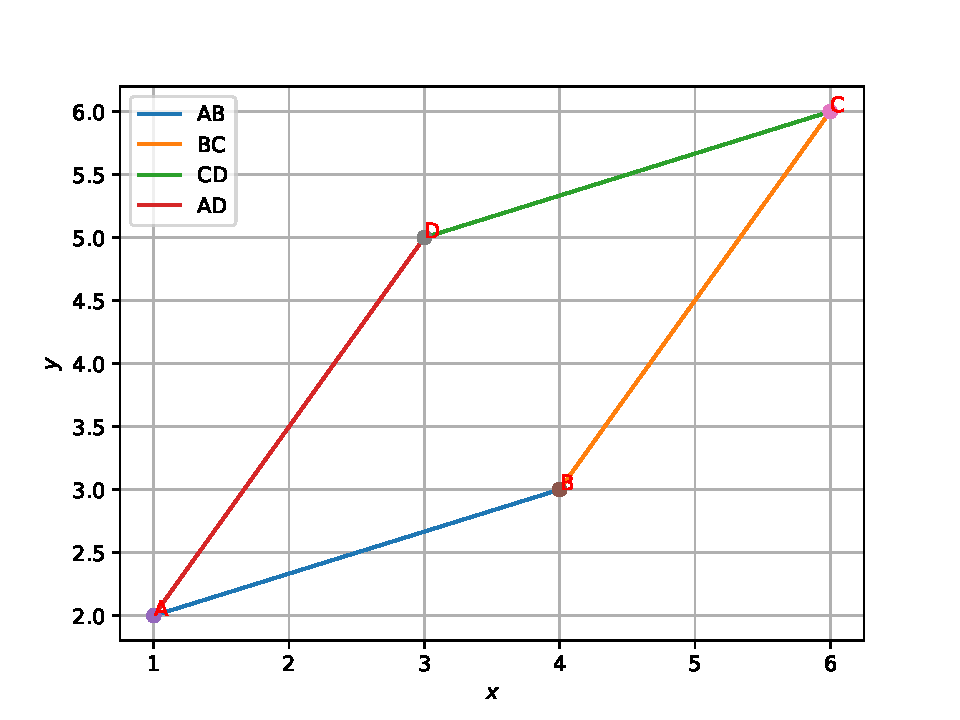
\includegraphics[width=\columnwidth]{./solutions/5/figs/lines/q10.eps}
	\caption{Parallelogram of Q.3.6.5}
	\label{fig:3.6.5_qten}	
	\end{figure}
	
		

\item If $\vec{A}=\myvec{-2\\-2}, \vec{B}=\myvec{2\\-4}$ respectively, find the coordinates of $\vec{P}$ such that $AP = \frac{3}{7}AB$ and $\vec{P}$ lies on the line segment $AB$.
\\
\solution
Let the balanced version of (\ref{eq:solutions/chem/6ato balance}) be
\begin{align}
    \label{eq:solutions/chem/6abalanced}x_{1}HNO_{3}+ x_{2}Ca(OH)_{2}\to x_{3}Ca(NO_{3})_{2}+ x_{4}H_{2}O
\end{align}

which results in the following equations:
\begin{align}
    (x_{1}+ 2x_{2}-2x_{4}) H= 0\\
    (x_{1}-2x_{3}) N= 0\\
    (3x_{1}+ 2x_{2}-6x_{3}- x_{4}) O=0\\
    (x_{2}-x_{3}) Ca= 0
\end{align}

which can be expressed as
\begin{align}
    x_{1}+ 2x_{2}+ 0.x_{3} -2x_{4} = 0\\
    x_{1}+ 0.x_{2} -2x_{3} +0.x_{4}= 0\\
    3x_{1}+ 2x_{2}-6x_{3}- x_{4} =0\\
    0.x_{1} +x_{2}-x_{3} +0.x_{4}= 0
\end{align}

resulting in the matrix equation
\begin{align}
    \label{eq:solutions/chem/6a matrix}
    \myvec{1 & 2 & 0 & -2\\
           1 & 0 & -2 & 0\\
           3 & 2 & -6 & -1\\
           0 & 1 & -1 & 0}\vec{x}
           =\vec{0}
\end{align}

where,
\begin{align}
   \vec{x}= \myvec{x_{1}\\x_{2}\\x_{3}\\x_{4}}
\end{align}

(\ref{eq:solutions/chem/6a matrix}) can be reduced as follows:
\begin{align}
    \myvec{1 & 2 & 0 & -2\\
           1 & 0 & -2 & 0\\
           3 & 2 & -6 & -1\\
           0 & 1 & -1 & 0}
    \xleftrightarrow[R_{3}\leftarrow \frac{R_3}{3}-R_{1}]{R_{2}\leftarrow R_2- R_1}
    \myvec{1 & 2 & 0 & -2\\
           0 & -2 & -2 & 2\\
           0 & -\frac{4}{3} & -2 & \frac{5}{3}\\
           0 & 1 & -1 & 0}\\
    \xleftrightarrow{R_2 \leftarrow -\frac{R_2}{2}}
    \myvec{1 & 2 & 0 & -2\\
          0 & 1 & 1 & -1\\
          0 & -\frac{4}{3} & -2 & \frac{5}{3}\\
          0 & 1 & -1 & 0}\\
    \xleftrightarrow[R_4 \leftarrow R_4- R_2]{R_3 \leftarrow R_3 + \frac{4}{3}R_2}
    \myvec{1 & 2 & 0 & -2\\
           0 & 1 & 1 & -1\\
           0 & 0 & -\frac{2}{3} & \frac{1}{3}\\
           0 & 0 & -2 & 1}\\
    \xleftrightarrow[R_3 \leftarrow -\frac{3}{2}R_3]{R_1 \leftarrow R_1- 2R_2}
    \myvec{1 & 0 & -2 & 0\\
           0 & 1 & 1 & -1\\
           0 & 0 & 1 & -\frac{1}{2}\\
           0 & 0 & -2 & 1}\\
    \xleftrightarrow{R_4\leftarrow R_4 + 2R_3}
    \myvec{1 & 0 & -2 & 0\\
           0 & 1 & 1 & -1\\
           0 & 0 & 1 & -\frac{1}{2}\\
           0 & 0 & 0 & 0}\\
    \xleftrightarrow[R_2\leftarrow R_2-R_3]{R_1\leftarrow R_1 + 2R_3}
    \myvec{1 & 0 & 0 & -1\\
           0 & 1 & 0 & -\frac{1}{2}\\
           0 & 0 & 1 & -\frac{1}{2}\\
           0 & 0 & 0 & 0}
\end{align}

Thus,
\begin{align}
    x_1=x_4, x_2= \frac{1}{2}x_4, x_3=\frac{1}{2}x_4\\
    \implies \quad\vec{x}= x_4\myvec{1\\ \frac{1}{2}\\ \frac{1}{2}\\1} =\myvec{2\\1\\1\\2}
\end{align} 
by substituting $x_4= 2$.

\hfill\break
%\vspace{5mm} 
Hence, (\ref{eq:solutions/chem/6abalanced}) finally becomes
\begin{align}
    2HNO_{3}+ Ca(OH)_{2}\to Ca(NO_{3})_{2}+ 2H_{2}O
\end{align}

\item Find the coordinates of the points which divide the line segment joining $\vec{A}=\myvec{-2\\2}, \vec{B}=\myvec{2\\8}$ into four equal parts.
\\
\solution
Let the balanced version of (\ref{eq:solutions/chem/6ato balance}) be
\begin{align}
    \label{eq:solutions/chem/6abalanced}x_{1}HNO_{3}+ x_{2}Ca(OH)_{2}\to x_{3}Ca(NO_{3})_{2}+ x_{4}H_{2}O
\end{align}

which results in the following equations:
\begin{align}
    (x_{1}+ 2x_{2}-2x_{4}) H= 0\\
    (x_{1}-2x_{3}) N= 0\\
    (3x_{1}+ 2x_{2}-6x_{3}- x_{4}) O=0\\
    (x_{2}-x_{3}) Ca= 0
\end{align}

which can be expressed as
\begin{align}
    x_{1}+ 2x_{2}+ 0.x_{3} -2x_{4} = 0\\
    x_{1}+ 0.x_{2} -2x_{3} +0.x_{4}= 0\\
    3x_{1}+ 2x_{2}-6x_{3}- x_{4} =0\\
    0.x_{1} +x_{2}-x_{3} +0.x_{4}= 0
\end{align}

resulting in the matrix equation
\begin{align}
    \label{eq:solutions/chem/6a matrix}
    \myvec{1 & 2 & 0 & -2\\
           1 & 0 & -2 & 0\\
           3 & 2 & -6 & -1\\
           0 & 1 & -1 & 0}\vec{x}
           =\vec{0}
\end{align}

where,
\begin{align}
   \vec{x}= \myvec{x_{1}\\x_{2}\\x_{3}\\x_{4}}
\end{align}

(\ref{eq:solutions/chem/6a matrix}) can be reduced as follows:
\begin{align}
    \myvec{1 & 2 & 0 & -2\\
           1 & 0 & -2 & 0\\
           3 & 2 & -6 & -1\\
           0 & 1 & -1 & 0}
    \xleftrightarrow[R_{3}\leftarrow \frac{R_3}{3}-R_{1}]{R_{2}\leftarrow R_2- R_1}
    \myvec{1 & 2 & 0 & -2\\
           0 & -2 & -2 & 2\\
           0 & -\frac{4}{3} & -2 & \frac{5}{3}\\
           0 & 1 & -1 & 0}\\
    \xleftrightarrow{R_2 \leftarrow -\frac{R_2}{2}}
    \myvec{1 & 2 & 0 & -2\\
          0 & 1 & 1 & -1\\
          0 & -\frac{4}{3} & -2 & \frac{5}{3}\\
          0 & 1 & -1 & 0}\\
    \xleftrightarrow[R_4 \leftarrow R_4- R_2]{R_3 \leftarrow R_3 + \frac{4}{3}R_2}
    \myvec{1 & 2 & 0 & -2\\
           0 & 1 & 1 & -1\\
           0 & 0 & -\frac{2}{3} & \frac{1}{3}\\
           0 & 0 & -2 & 1}\\
    \xleftrightarrow[R_3 \leftarrow -\frac{3}{2}R_3]{R_1 \leftarrow R_1- 2R_2}
    \myvec{1 & 0 & -2 & 0\\
           0 & 1 & 1 & -1\\
           0 & 0 & 1 & -\frac{1}{2}\\
           0 & 0 & -2 & 1}\\
    \xleftrightarrow{R_4\leftarrow R_4 + 2R_3}
    \myvec{1 & 0 & -2 & 0\\
           0 & 1 & 1 & -1\\
           0 & 0 & 1 & -\frac{1}{2}\\
           0 & 0 & 0 & 0}\\
    \xleftrightarrow[R_2\leftarrow R_2-R_3]{R_1\leftarrow R_1 + 2R_3}
    \myvec{1 & 0 & 0 & -1\\
           0 & 1 & 0 & -\frac{1}{2}\\
           0 & 0 & 1 & -\frac{1}{2}\\
           0 & 0 & 0 & 0}
\end{align}

Thus,
\begin{align}
    x_1=x_4, x_2= \frac{1}{2}x_4, x_3=\frac{1}{2}x_4\\
    \implies \quad\vec{x}= x_4\myvec{1\\ \frac{1}{2}\\ \frac{1}{2}\\1} =\myvec{2\\1\\1\\2}
\end{align} 
by substituting $x_4= 2$.

\hfill\break
%\vspace{5mm} 
Hence, (\ref{eq:solutions/chem/6abalanced}) finally becomes
\begin{align}
    2HNO_{3}+ Ca(OH)_{2}\to Ca(NO_{3})_{2}+ 2H_{2}O
\end{align}

%\end{enumerate}
%
